% generated by scripts/pkl_to_latex.py
% source PKL : uscan_v1_L8_Ne6_t1_mode-uniform_nmin2_solver-gcg_sz0_restarts10_iter300_kmax4_tol1em09_U1to20_N20-d03a74da789e.pkl
% scan type  : uscan
% state      : gs
% quantity   : purity
% requires   : \usepackage{pgfplots} \pgfplotsset{compat=1.18}
% colours match the matplotlib PDF (tab10 cycle)
\definecolor{gmeC0}{HTML}{1F77B4}
\definecolor{gmeC1}{HTML}{FF7F0E}
\definecolor{gmeC2}{HTML}{2CA02C}
\definecolor{gmeC3}{HTML}{D62728}
\definecolor{gmeC4}{HTML}{9467BD}
\definecolor{gmeC5}{HTML}{8C564B}
\definecolor{gmeC6}{HTML}{E377C2}
\definecolor{gmeC7}{HTML}{17BECF}

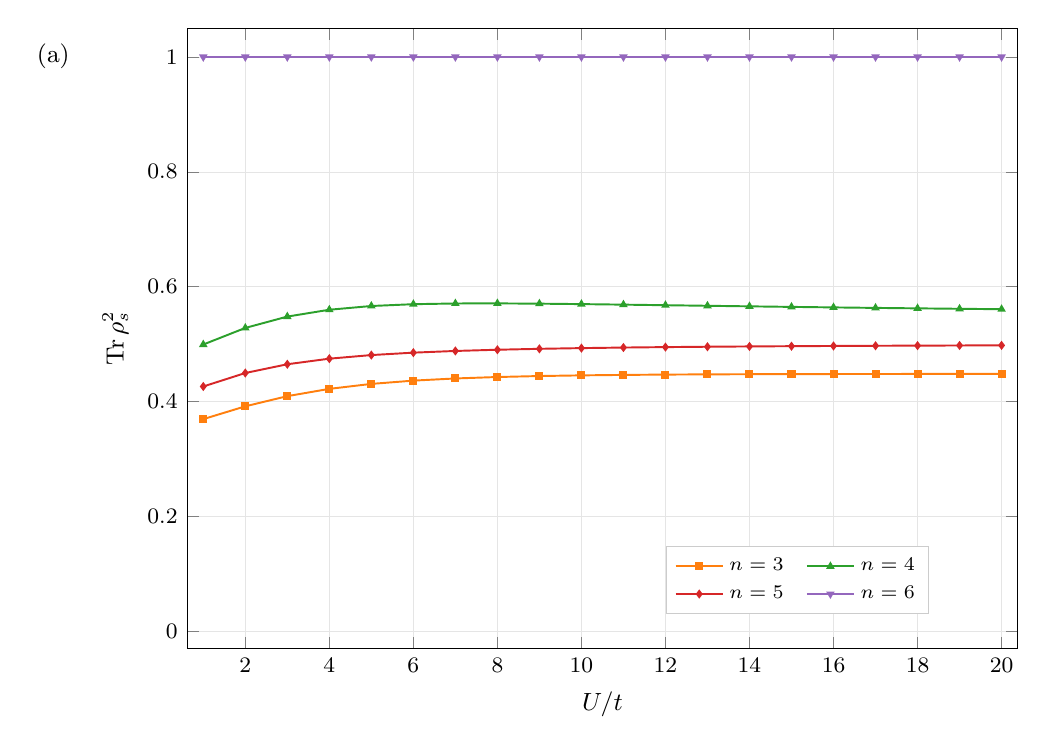
\begin{tikzpicture}
  \begin{axis}[
    width=\columnwidth,
    height=0.78\columnwidth,
    xlabel={$U/t$},
    ylabel={$\mathrm{Tr}\,\rho_s^2$},
    grid=both,
    grid style={line width=.1pt, draw=gray!20},
    tick label style={font=\footnotesize\rmfamily, /pgf/number format/fixed},
    label style={font=\small\rmfamily},
    scaled ticks=false,
    legend style={font=\scriptsize\rmfamily, draw=gray!40, at={(0.5,1.03)}, anchor=south, /tikz/every even column/.append style={column sep=6pt}},
    legend cell align={left},
    legend columns=2,
    ymin=-0.03,
    ymax=1.05,
    xmin=0.62,
    xmax=20.38,
    legend style={at={(0.735,0.110)}, anchor=center, fill=white},
    after end axis/.append code={\node[anchor=east, font=\small\rmfamily] at (axis description cs:-0.13,0.954) {(a)};},
  ]
    \addplot[color=gmeC1, mark=square*, mark size=1.1pt, line width=0.7pt] coordinates {
        (1,0.369259) (2,0.391577) (3,0.409265) (4,0.421976)
        (5,0.430599) (6,0.436311) (7,0.440085) (8,0.442601)
        (9,0.444299) (10,0.445461) (11,0.446264) (12,0.446823)
        (13,0.447213) (14,0.447484) (15,0.44767) (16,0.447794)
        (17,0.447873) (18,0.44792) (19,0.447941) (20,0.447944)
    };
    \addlegendentry{$n=3$}
    \addplot[color=gmeC2, mark=triangle*, mark size=1.1pt, line width=0.7pt] coordinates {
        (1,0.499183) (2,0.528068) (3,0.547827) (4,0.559754)
        (5,0.56626) (6,0.569424) (7,0.57065) (8,0.570787)
        (9,0.570327) (10,0.569552) (11,0.568624) (12,0.567633)
        (13,0.566633) (14,0.565653) (15,0.564709) (16,0.563808)
        (17,0.562955) (18,0.562149) (19,0.56139) (20,0.560676)
    };
    \addlegendentry{$n=4$}
    \addplot[color=gmeC3, mark=diamond*, mark size=1.1pt, line width=0.7pt] coordinates {
        (1,0.426124) (2,0.449568) (3,0.464833) (4,0.474544)
        (5,0.480823) (6,0.485031) (7,0.487968) (8,0.490098)
        (9,0.491696) (10,0.492928) (11,0.4939) (12,0.494681)
        (13,0.49532) (14,0.495849) (15,0.496292) (16,0.496668)
        (17,0.496988) (18,0.497265) (19,0.497505) (20,0.497714)
    };
    \addlegendentry{$n=5$}
    \addplot[color=gmeC4, mark=triangle*, mark size=1.1pt, mark options={rotate=180}, line width=0.7pt] coordinates {
        (1,1) (2,1) (3,1) (4,1)
        (5,1) (6,1) (7,1) (8,1)
        (9,1) (10,1) (11,1) (12,1)
        (13,1) (14,1) (15,1) (16,1)
        (17,1) (18,1) (19,1) (20,1)
    };
    \addlegendentry{$n=6$}
  \end{axis}
\end{tikzpicture}
